\documentclass{book}
\usepackage{tikz}
\usetikzlibrary{positioning,arrows.meta,fit}
\begin{document}
    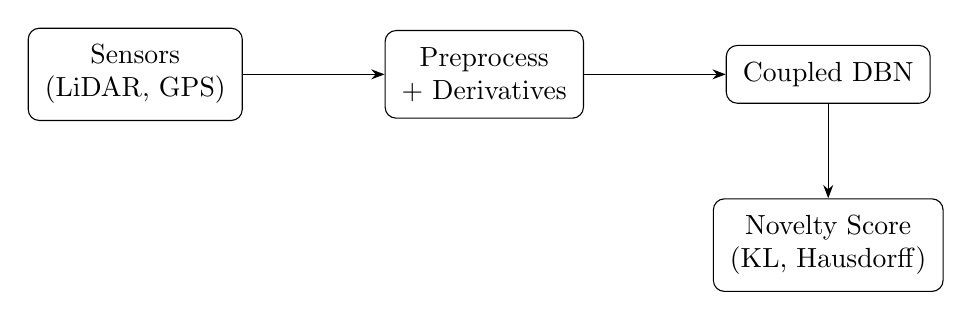
\begin{tikzpicture}[
        box/.style={draw, rounded corners, align=center, inner sep=6pt},
        >=Stealth]
        \node[box] (sense) {Sensors\\(LiDAR, GPS)};
        \node[box, right=18mm of sense] (features) {Preprocess\\ + Derivatives};
        \node[box, right=18mm of features] (model) {Coupled DBN};
        \node[box, below=12mm of model] (novel) {Novelty Score\\(KL, Hausdorff)};
        \draw[->] (sense) -- (features);
        \draw[->] (features) -- (model);
        \draw[->] (model) -- (novel);
    \end{tikzpicture}
\end{document}